% -----------------------------------------------------------------
% Document class: Article
\documentclass[ a4paper, twoside, 11pt]{article}
\usepackage{../../../macros-general}
\usepackage{../../../macros-article}
% Number of the handout, quiz, exam, etc.
\newcommand{\numero}{05}
\setcounter{numero}{\numero}

% -----------------------------------------------------------------
\begin{document}
\allowdisplaybreaks

\begin{center}
\Large Mec\'anica Vectorial (MECG-1001): Trabajo Aut\'onomo \numero \\[2ex]
\small \textbf{Semestre:} 2017-2018 T\'ermino II \qquad
\textbf{Instructor:} Luis I. Reyes Castro \qquad
\textbf{Paralelo:} 09
\end{center}
\fullskip

% =============================================
\begin{problem}
\textbf{[4 Puntos]} Cada uno de los engranes $A$ y $B$ pesa 20 lbs y tiene un radio de giro de 7.5 in; el engrane $C$ pesa 5 lb y tiene un radio de giro de 3 in. Si un par $M$ de magnitud constante de 50 lb-in se aplica al engrane $C$, determine \textit{(i)} la aceleraci\'on angular del engrane $A$, \linebreak \textit{(ii)} la fuerza tangencial que ejerce el engrane $C$ sobre el engrane $A$.

\begin{figure}[htb]
\centering
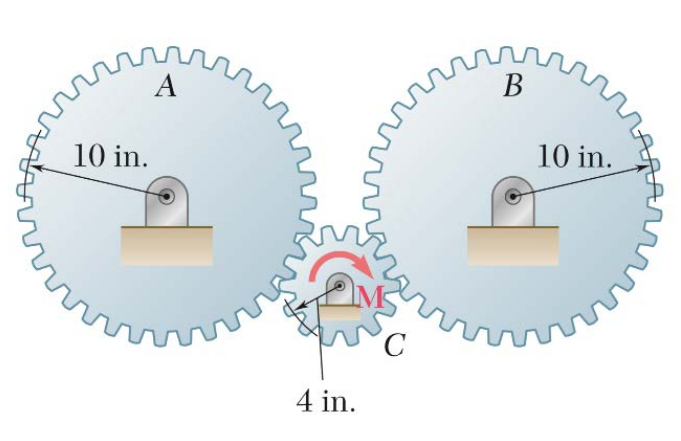
\includegraphics[width=0.4\textwidth]{problema-1.jpg}
\end{figure}

\end{problem}
\fullskip

% =============================================
\begin{problem}
\textbf{[4 Puntos]} Una barra ligera de 1.5 kg est\'a soldada a un disco uniforme de 5 kg en la forma que se muestra. El ensamble oscila libremente alrededor de $C$ en un plano vertical. Si en la posici\'on indicada el ensamble es liberado con una velocidad angular de 10 rad/s \linebreak en direcci\'on de las manecillas del reloj, determine \textit{(i)} la aceleraci\'on angular del ensamble, \linebreak \textit{(ii)} las componentes de la reacci\'on en $C$. 

\begin{figure}[htb]
\centering
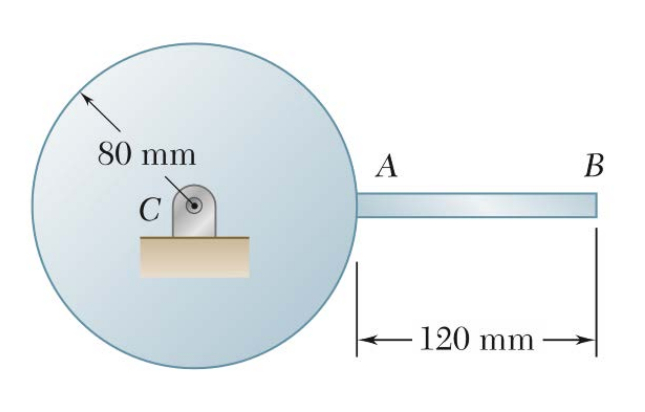
\includegraphics[width=0.4\textwidth]{problema-2.jpg}
\end{figure}

\end{problem}
\fullskip

\end{document}